\noindent
\section{Forming reviewer groups}
\label{group}

The results in the previous section together lead us to believe that the editors in numerous cases fail to assign reviewers which may further lead to flawed papers 
being accepted into the literature while at 
the same time quality research being overlooked. We hence proceed to propose a framework that could recommend compatible referee groups which could then be assigned to 
a submitted paper. 
Note that such a system would be required to - \\
(i) recommend multiple items (referees) to a single user (submission).\\ 
(ii) recommend only homogeneous (compatible) items together while making multiple recommendations. \\ 
(iii) provide a scheme to rank the groups since there could be numerous compatible groups and recommending all of them would be infeasible. \\
Genetic algorithm has already been found to be very effective in obtaining desired groups in collaborative learning setting \cite{moreno2012genetic,ani2010method} 
and we argue that assigning multiple referees to a submission is similar to forming 
compatible referee groups. More importantly, for such a framework a scheme for ranking the groups is inherently present (we provide a detailed description later in this section).   
We hence leverage the idea of GA based team formation framework to obtain the best possible combination of referees which might lead to better judgment of the quality 
of the work. 
%In specific, we use a genetic algorithm framework to obtain the best possible referee assignments for a given paper. Note 
%\mycheck{why GA?}

%hence we leverage this framework to obtain the best possible multiple-referee assignments for a given paper.

\subsection{Problem definition} Given a submission $S$, a set of reviewers $R = \{R_1, R_2,\ldots, R_n\}$ and the number 
of reviewers to be assigned for a paper $k$, the goal is to obtain a set of potential reviewer groups $G = \{ G_1, G_2, \ldots, G_u\}$ (each of size $k$) 
who could be assigned to referee a submission.

\subsection{Methodology}
We now proceed to develop a solution to the above problem based on a genetic algorithm framework which is inspired by the method proposed in~\cite{ani2010method}. 
Typically, chromosomes are represented as simple
strings of data and instruction. In our case chromosomes represent solutions while reviewers are chosen as genes. The details of our algorithm is as follows -- 
\subsubsection{Selecting a population} Genetic algorithm starts with an initial population represented by the chromosomes. 
Ideally the assigned reviewers should be knowledgeable and experienced in the topics related to the submitted paper. Although information about the associated topic of the papers are not present, each paper in the dataset is  associated with a set of keywords (at least 1 and at most 4, assigned by the publisher) which we use as a proxy for the topic. While the JHEP dataset consists of 201 unique keywords, JSTAT dataset has 562. This again indicates that the papers in JSTAT are more diverse. 
Hence for  a given 
submission we first extract the keywords. 
%As mentioned earlier the keywords are used as a proxy for the topic of the paper. Note that a better way would be to explicitly obtain the topic of the paper, but due to lack of information we use the keywords. In case the topics are explicitly available, it can be easily incorporated into our framework. 
Given the keywords, we extract from the pool of referees only those peers who have reviewed, till the date of the submission in question, at least one paper 
that has one (or more) keywords in common with that of the submission. This set ($\bar R$) represents the potential population of reviewers for the query paper.

% \begin{figure}
%  \centering
%  \includegraphics[scale = 0.26]{figures/topic.eps}
%  \caption{\label{topic} Cumulative distribution function of the fraction of papers being multi-refereed across all the keywords for both JHEP and JSTAT datasets.}
% \end{figure}


\subsubsection{Initialization} Once the initial population $\bar R$ of reviewers is obtained, we classify them based on 
the accept ratio and time from the last assignment. For each reviewer $i$ we obtain the accept ratio $a_{i}$ and time from the last 
assignment $d_i$ (scaled between 0 and 1). Finally, we calculate the fitness score for the reviewer $i$ as -
\begin{equation}
 f_i = \alpha \ast a_i + (1-\alpha)\ast d_i
\end{equation}
where $\alpha$ is a tuning parameter. Based on the fitness score we classify each reviewer into one of the three classes. Reviewers with fitness score 
less than $0.33$ are classified as class 1 ($RC_1$), between $0.33$ and $0.66$ are classified as class 2 ($RC_2$) and the rest as class 3 ($RC_3$). 
We then club the reviewers randomly into non-overlapping groups of size $k$. This forms the initial generation with each group represented as 
a chromosome. Note that a generation forms a solution set for the above problem.

\subsubsection{Fitness evaluation}
Once a generation is obtained, we proceed to calculate the fitness of each chromosome (group) and, thereby, calculate the fitness of the whole generation. 
The generation level fitness ($FG_{gen}$) is calculated according to function 1 for a generation $gen$. For each class $RC_i$ we initially calculate the number of reviewers in $RC_i$ 
per group (represented by $RPC_i$). Now for every group $g_j$ we find the number of reviewers of each class $RC_i$  which we represent by $RC_{i}^{g_j}$. We penalize the 
chromosome if the constraint (refer to line 10 of function 1) is violated by not adding anything to the final score; otherwise, a value of 1000 is added to the fitness score.
Note that $1000$ is a representative value and for practical purposes we can use any positive value ($C$). 
More importantly this scoring scheme further allows for ranking the groups. 
\begin{function1}
 \caption{generation\_level\_fitness()}
 $G$, $RC_i$ \\ 
 $FG_{gen} \leftarrow$ 0\\
 $|G|\leftarrow$ Number of groups\\
 $|RC_i|\leftarrow$ Number of peers in $RC_i$\\
 $|RPC_i|\leftarrow$ Number of peers of class $RC_i$ per group (i.e., $|RPC_i| = |RC_i|/|G|$) \\
 $|RC_{i}^{g_j}|\leftarrow$ Number of actual peers of class $RC_{i}$ in $g_j$\\
 \For{each group $g_j \in G$}{
 \For{each $RC_i$}{
 \If{$|RC_{i}^{g_j}|\geq |RPC_i|$}{
  $FG_{gen} = FG_{gen} + 1000$\\
      } 
    }
 }
 \Return{$FG_{gen}$}
\end{function1}
%\vspace{-8mm}
%\mycheck{An example to illustrate the computation of the above fitness would be nice.Sandipan: added}

To illustrate on how the fitness function is calculated we consider here a toy example. Consider a population of 16 reviewers (with ids 0 - 15), group size of 4 and 3 reviewer classes (1, 2, 3) with number of reviewers in each class being 6, 5 and 5 respectively. Let the reviewers with ids 0 - 5 are assigned to class 1, 6 - 10 to class 2 and rest are assigned to class 3. 
So, $|RPC_1| = 1.5$, $|RPC_2| = 1.25$ and $|RPC_3| = 1.25$.
%\mycheck{The calculation is not correct. Check $|RPC_3| = 1.25$} 
Each generation consists of 4 groups. Let us consider a group $g$ with reviewers 0, 1, 6 and 12. For this group  $|RC_1^{g}| = 2$, $|RC_2^{g}| = 1$ and $|RC_3^{g}| = 1$. Since $|RC_1^{g}| > RPC_1$, it contributes a score of 1000. Similarly $|RC_2^{g}|$ and $|RC_3^{g}|$ does not contribute to any score. 
%\mycheck{According to your example $|RC_3^{g}| < |RPC_3|$ and therefore should not add a score of 1000. CHECK.} 
Hence the score contributed by this group to the generation is 1000. Sum of this score across all the groups in the generation equals the generation level fitness. 
Note that our algorithm is inherently fair because the proportion of referees in each class is maintained in the recommended set of referees.

\subsubsection{Crossover}
Crossover is the process in which two chromosomes combine the genetic material to create a new generation such that the new one possesses the genetic material of both. 
Although several techniques for crossover exist~\cite{golberg1989genetic}, we here consider the one-point crossover technique. 
One random position in the chromosome is chosen to determine the crossover point. In the offsprings produced, the data till the crossover point are copied verbatim from the parents while the data beyond the crossover point are swapped between the two parents. As a result, these new chromosomes or
offsprings share some similar features from the parents chosen. If the crossover is not applied, offsprings are exact copies
of the parents. We have set the crossover rate for our experiments to 70\%. 
Note that mutation process can also be used to maintain genetic diversity but we only stick to crossover for our experiments. 
The process of crossover is repeated several times and the fitness score of the generation is calculated each time. The generation 
with the best score is confirmed as the best possible reviewer grouping for the submitted paper.

\begin{figure}
\centering
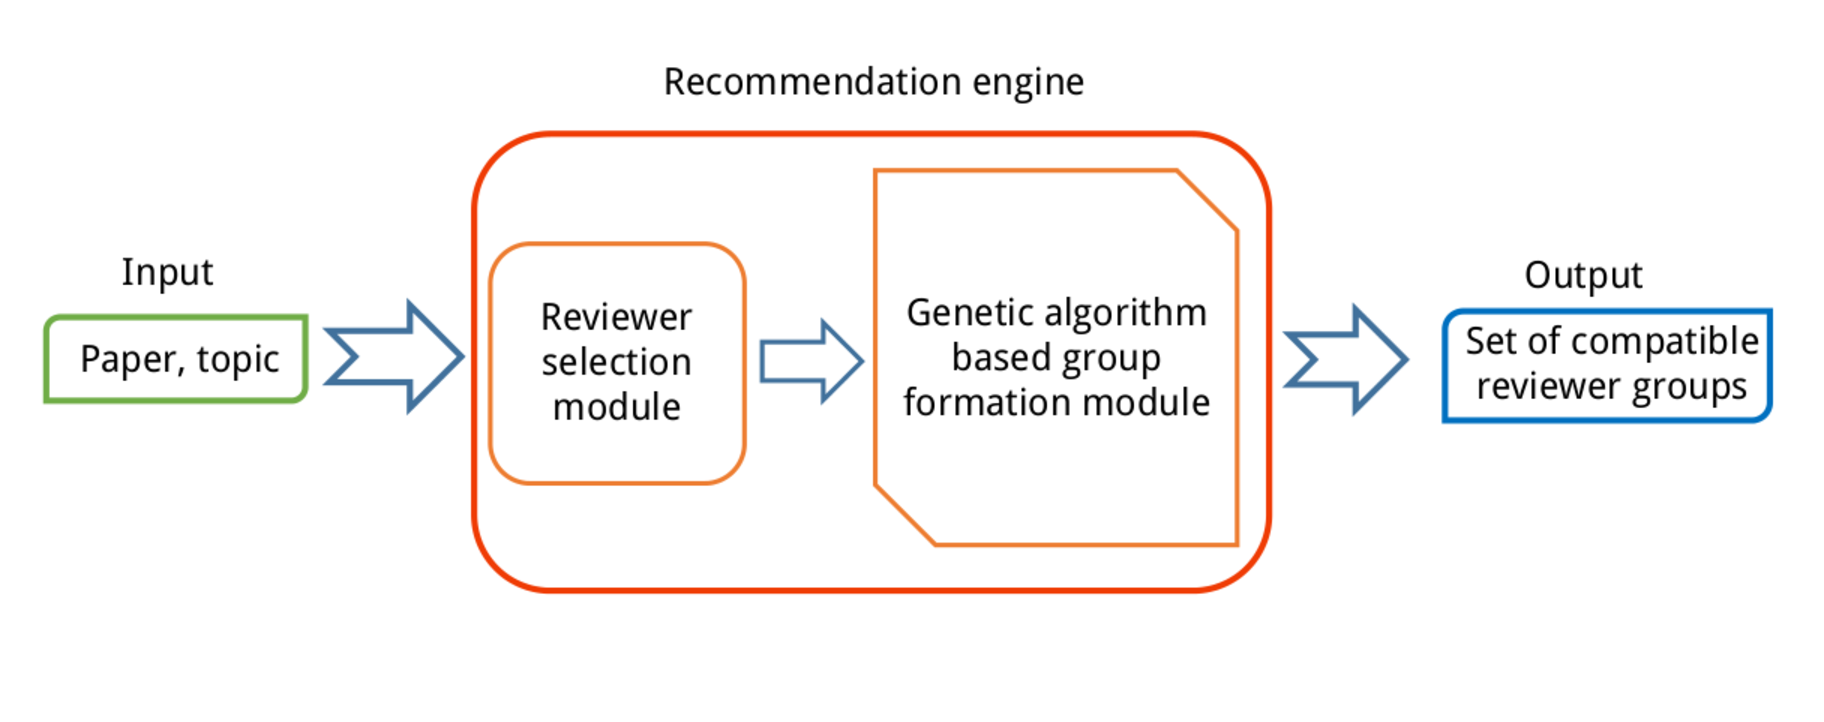
\includegraphics[scale=0.32]{./texfiles/Chapter_4/cikm_17/figures/r_d_g.pdf}
\caption{\label{r_d_g} Block diagram demonstrating the work flow of our system.}
\end{figure}

\subsection{Evaluation}

To evaluate the performance of our algorithm, we initially separate out the multi-refereed papers from both the datasets. Based on the long term citations received by each, 
we classify them as high and low cited. Specifically we rank them based on their citations and top 25 percentile are classified as highly cited ones and bottom 25 percentile 
are classified as low cited ones. The classification is done separately across both accepted and rejected papers. We hypothesize that - \\
(i) For accepted papers, highly cited papers represent the cases where the reviewer group was chosen correctly. Moreover, if the reviewer group which was originally assigned 
the paper is also one of the groups recommended by our algorithm, we consider it as a true positive case.\\
(ii) Similarly for rejected papers, low cited papers also represent the cases where the reviewer group was chosen correctly and if our recommendation matches we consider 
it as true positive as well.\\
(iii) For accepted papers, low cited papers represent the cases where the reviewer group was not chosen correctly. If for such a paper the original reviewer group does not feature in the 
list of recommended groups, we consider it as true negative. \\ 
(iv) Similarly, for rejected papers, high cited papers also represent the cases where the reviewer group was not chosen correctly and our hypothesis follows. \\
Since our algorithm allows for ranking of the groups based on the fitness score, we recommend top $k$ (how the results vary with $k$ is shown later) percentile groups. A block diagram representing the work flow of our system is presented in figure \ref{r_d_g}.
%Note that we recommend top $k$ percentile instead of recommending a fixed number as in traditional case. This is because the candidate set of groups is not fixed and grows with 
%time.

% \begin{figure}
% \centering
% 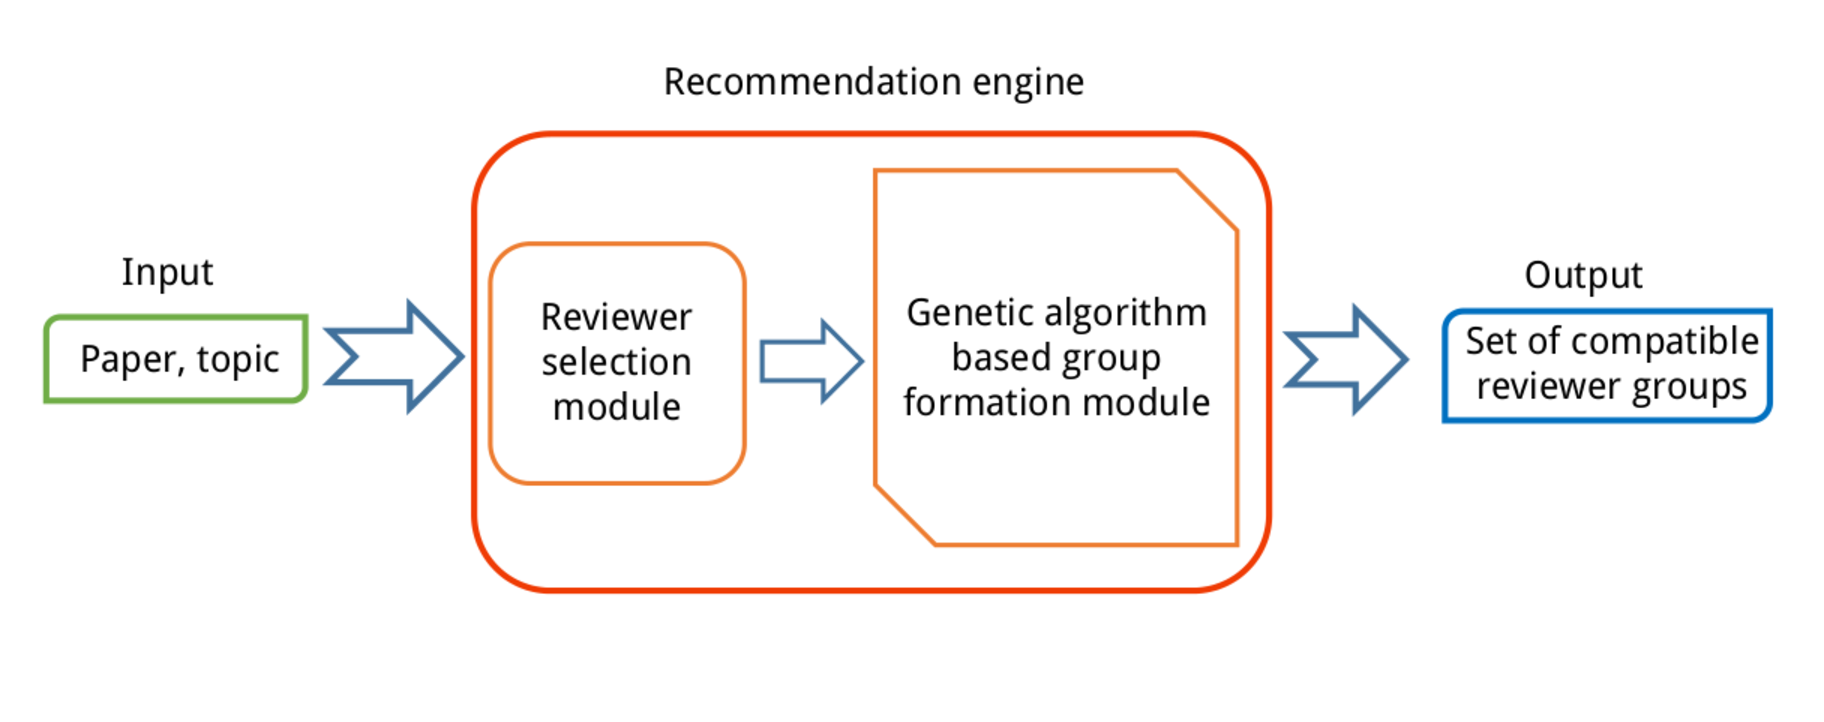
\includegraphics[scale=0.32]{./texfiles/Chapter_4/cikm_17/figures/r_d_g.pdf}
% \caption{\label{r_d_g} Block diagram demonstrating the work flow of our system.}
% \end{figure}

%\mycheck{put in the parameter estimation values}

\noindent{\bf Sensitivity to the parameters:}
As mentioned earlier, our algorithm requires two parameters, (i) $\alpha$ and (ii) the crossover rate. In figure~\ref{fig:param_estimte}(a) we plot the true positive rate 
for different values of $\alpha$. We observe that TP (averaged over accepted and rejected cases) improves with increasing value of $\alpha$ after which it drops for 
both JHEP and JSTAT datasets. Optimal result is obtained at $\alpha = 0.6$ for JHEP and $\alpha = 0.7$ for JSTAT. 
We hence set the value of $\alpha$ at 0.6 and 0.7 respectively for JHEP and JSTAT datasets. \\
We further look into the crossover rate as well. In figure~\ref{fig:param_estimte}(b), we plot TP for different crossover rates. TP is observed to be lower for 
low crossover rate. This is because lower crossover rate allows for very low change of the chromosomes and since we set the number of generations to a constant  On the other hand, for very high crossover rate changes in the chromosome occurs at higher rates which increases the chances of obtaining the best solution. 
Optimal TP is obtained at 70\% crossover rate and hence we set the crossover rate at $70\%$ for our experiments. The number of generations we examine is set at 500.\\ 
\noindent{\bf Key results:}  
For both JHEP and JSTAT mostly two reviewers are assigned per submission albeit there are cases where three reviewers have also been assigned. 
For generating the results, we only consider the cases where the number of assigned reviewers were two. We calculate for each reviewer the accept ratio and time from the last assignment at the point of submission. 
We then run our algorithm for each submission falling in highly cited and low cited accepted and rejected papers. 
Note that we rank the papers based on citations it has accrued and consider the top and bottom 25 percentile 
to be high and low cited papers respectively. 
%25 percentile category. \mycheck{This is misleading? 25 percentile category of WHAT? Nothing is clear.} 
In table~\ref{tab:k} we present the true positive and true negative values for both JSTAT and JHEP at different values of $k$ (note that we rank the groups based 
on the fitness score and recommend groups in the top $k$ percentile). 
With $k = 15$, for JHEP we could recommend the correct group of reviewers in $81\%$ 
of the cases (represented by the true positive value) for accepted papers and $75\%$ of the cases for rejected papers. Similarly, we could correctly identify $84\%$ of the true negative cases for the accepted papers and $73\%$ for the rejected papers. Corresponding values for JSTAT are 
$79\%$ (accepted), $75\%$ (rejected) and $81\%$ (accepted), $71\%$ (rejected) respectively. %\mycheck{I think you can also report MRR. Can we report NDCG also?} 
These results indicate that our algorithm is indeed very effective in recommending referee pairs. We further look into the cases where 
our algorithm failed to obtain the correct grouping. We observe that in most of these cases a new reviewer (without any previous review history) was assigned. 
Since our algorithm recommends reviewers leveraging the review history, these cases were missed.
%For cases where three reviewers were assigned, our algorithm could correctly recommend at least two referees in 
%$73\%$ cases on average across accepted and rejected papers for JHEP and $69\%$ for JSTAT. 
We further check our results for $k=5$ and $k=10$ which are also reported in 
table~\ref{tab:k}. With $k=5$ we were able to obtain TP of 0.61 and 0.59 respectively for accepted and rejected papers in case of JHEP. For JSTAT the corresponding values 
are 0.63 and 0.59. More importantly we could obtain a high TN of 0.91 (accepted) and 0.89 (rejected) for JHEP and 0.92, 0.82 for JSTAT. This is because we are 
recommending a smaller number of groups which reduces the possibility of recommending a particular undesired/desired group.\\
\noindent{\bf Comparison with baseline algorithms:} %\mycheck{rewrite the baseine algorithm..}
As our algorithm presents computational overhead a natural question to ask is whether it is worth it. We hence design a simple 
baseline (random) to compete with our algorithm. For a submission, initial population of suitable reviewers is obtained (in the same way as our GA based algorithm) and each reviewer is classified into one of L, M, H categories. A subset of reviewers is then selected randomly in such a way that the proportion of reviewers in each class (in the population) is maintained 
in the chosen set. 
We then randomly form groups of types MM, ML and MH since these are the best performing reviewer groups (refer to figure \ref{ref_perf}).  
To compare, we obtain the same number of groups as obtained from our proposed algorithm. 
%hence we check if the originally assigned group of reviewers is present 
%in the recommended set (which is considerably larger than our recommended set since all random pairings of referees are part of this set). 
We further consider two other 
ablation type baselines - (i) GA with only accept ratio (only $a_i$, fitness score is calculated with only $a_i$), (ii) GA with only time since last assignment 
(only $d_i$, fitness score calculated with only $d_i$). Note that this can be achieved by setting $\alpha$ to 1 and 0 respectively. 
In figure~\ref{fig:GA_base} we plot the TP and TN for 
the baseline algorithms and our proposed algorithm ($k$ is set at 15). 
We consider five random instances and report the mean value for the baseline. We observe TP (averaged over accepted and rejected cases) 
to be much lower (0.37 (JHEP) and 0.45 (JSTAT) for random, 0.51 and 0.53 for only $a_i$, 0.42 and 0.37 for only $d_i$) compared to our algorithm. 
 TN is compared to be higher because of the less possibility of randomly obtaining a particular undesired/desired group.  
As a second level of evaluation we further consider overlap in the set of groups proposed by our 
algorithm with those obtained from the baseline algorithm. The purpose of this is to show that the top $k$ groups proposed by our algorithm based on the fitness function cannot be obtained 
through random allocation. In specific, we measure the Jaccard similarity between the set of groups obtained through baseline and those obtained through our algorithm. Across 
all the papers we obtain a low similarity value of 0.31 which further corroborates our hypothesis.\\
%\mycheck{Two other ablation type baselines could be: Our GA framework with the fitness score calculated base on (i) only accept ratio and (ii) time since last assignment.}
\begin{figure}
\centering
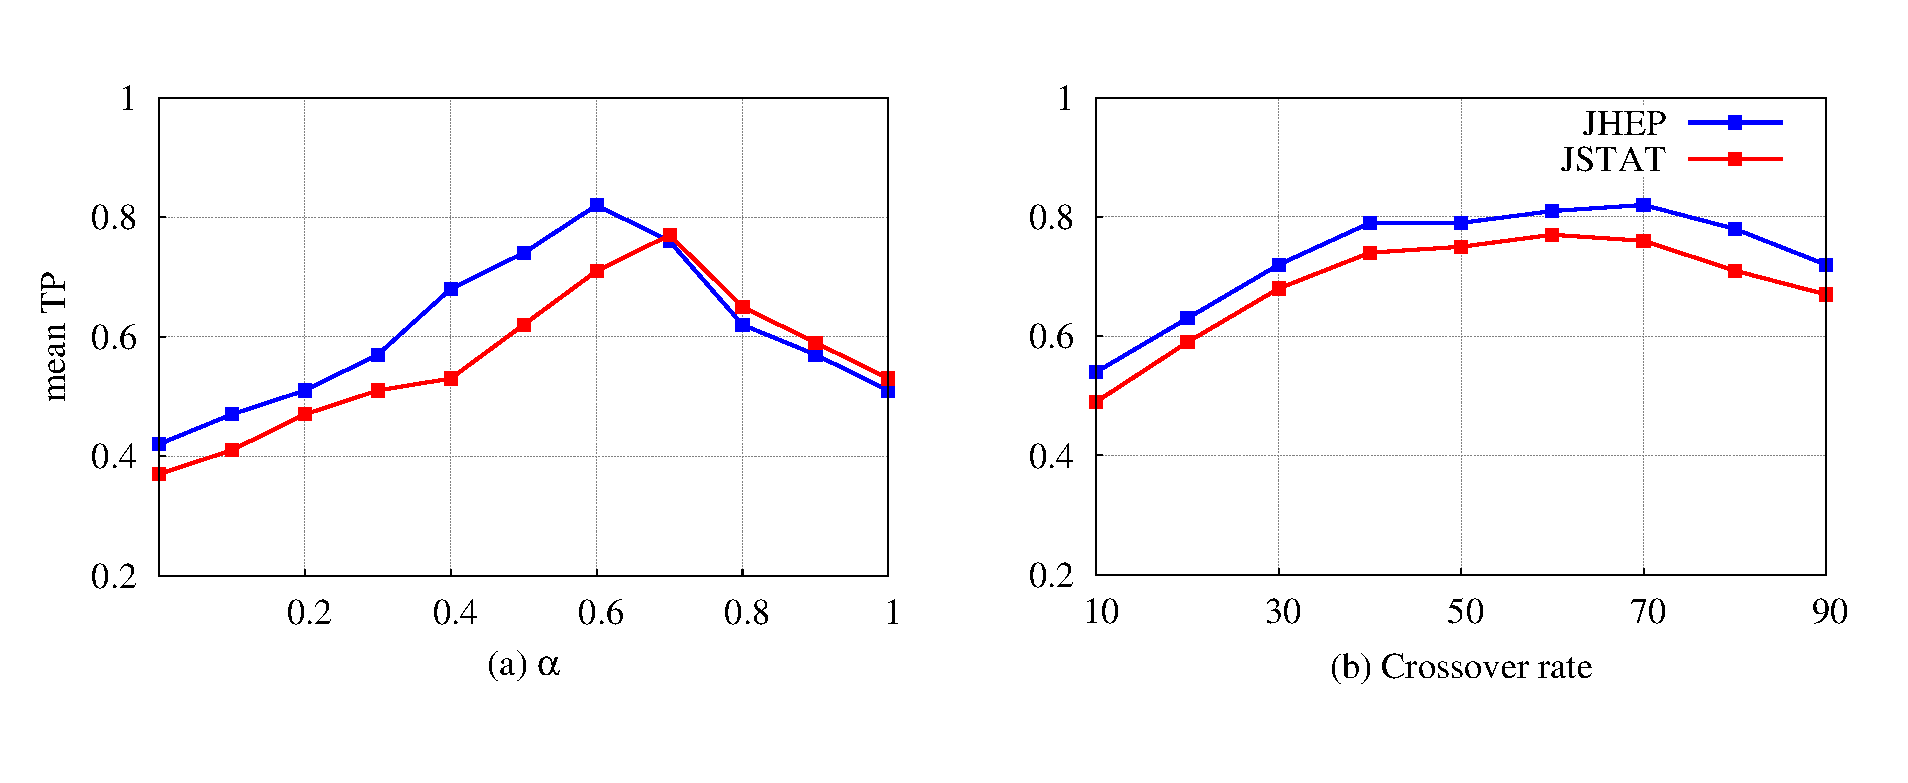
\includegraphics[scale = 0.35]{./texfiles/Chapter_4/cikm_17/figures/param_estimate.eps}
\caption{\label{fig:param_estimte} Mean true positive (averaged over accepted and rejected papers) value while recommending a set of reviewer groups for papers across different values 
of (a) $\alpha$ and (b) crossover rate. Experiments repeated for both JHEP and JSTAT datasets. $k = 15$}
\end{figure}


\begin{table}[]
\centering
\caption{True positive (TP) and true negative (TN) values across accepted and rejected papers measured for different values of $k$. Results are reported for JHEP and JSTAT datasets.}
\label{tab:k}
%\resizebox{!}{1.5cm}{
\begin{tabular}{c|c c|c c}
\hline
        & \multicolumn{2}{c|}{JHEP}                                                                                                   & \multicolumn{2}{c}{JSTAT}                                                                                                  \\ \hline
K       & \begin{tabular}[c]{@{}c@{}}TP\\ (accept,reject)\end{tabular} & \begin{tabular}[c]{@{}c@{}}TN\\ (accept,reject)\end{tabular} & \begin{tabular}[c]{@{}c@{}}TP\\ (accept,reject)\end{tabular} & \begin{tabular}[c]{@{}c@{}}TN\\ (accept,reject)\end{tabular} \\ \hline
5       &  0.61,0.59                                                   &  0.91,0.87                                                   &   0.63,0.59                                                  & 0.92,0.82                                                             \\ 
10      &  0.72,0.66                                                   &  0.87,0.79                                                   &   0.73,0.71                                                  & 0.85,0.76                                                             \\ 
15      &  0.81,0.75                                                   &  0.84,0.73                                                   &   0.79,0.74                                                  & 0.81,0.71                                                             \\ \hline \hline
Average &  0.71,0.66                                                   &  0.87,0.80                                                   &   0.72,0.68                                                  & 0.86,0.76                                                             \\ \hline
\end{tabular}%}
\end{table}
%\begin{figure}
%\includegraphics[scale = 0.26]{figures/G_A_all.eps}
%\caption{\label{fig:G_A} True positive (TP) and true negative (TN) cases while recommending a set of reviewer groups for both accepted and rejected papers for (a) JHEP and (b) JSTAT datsets.}
%\end{figure}



\begin{figure}
\centering
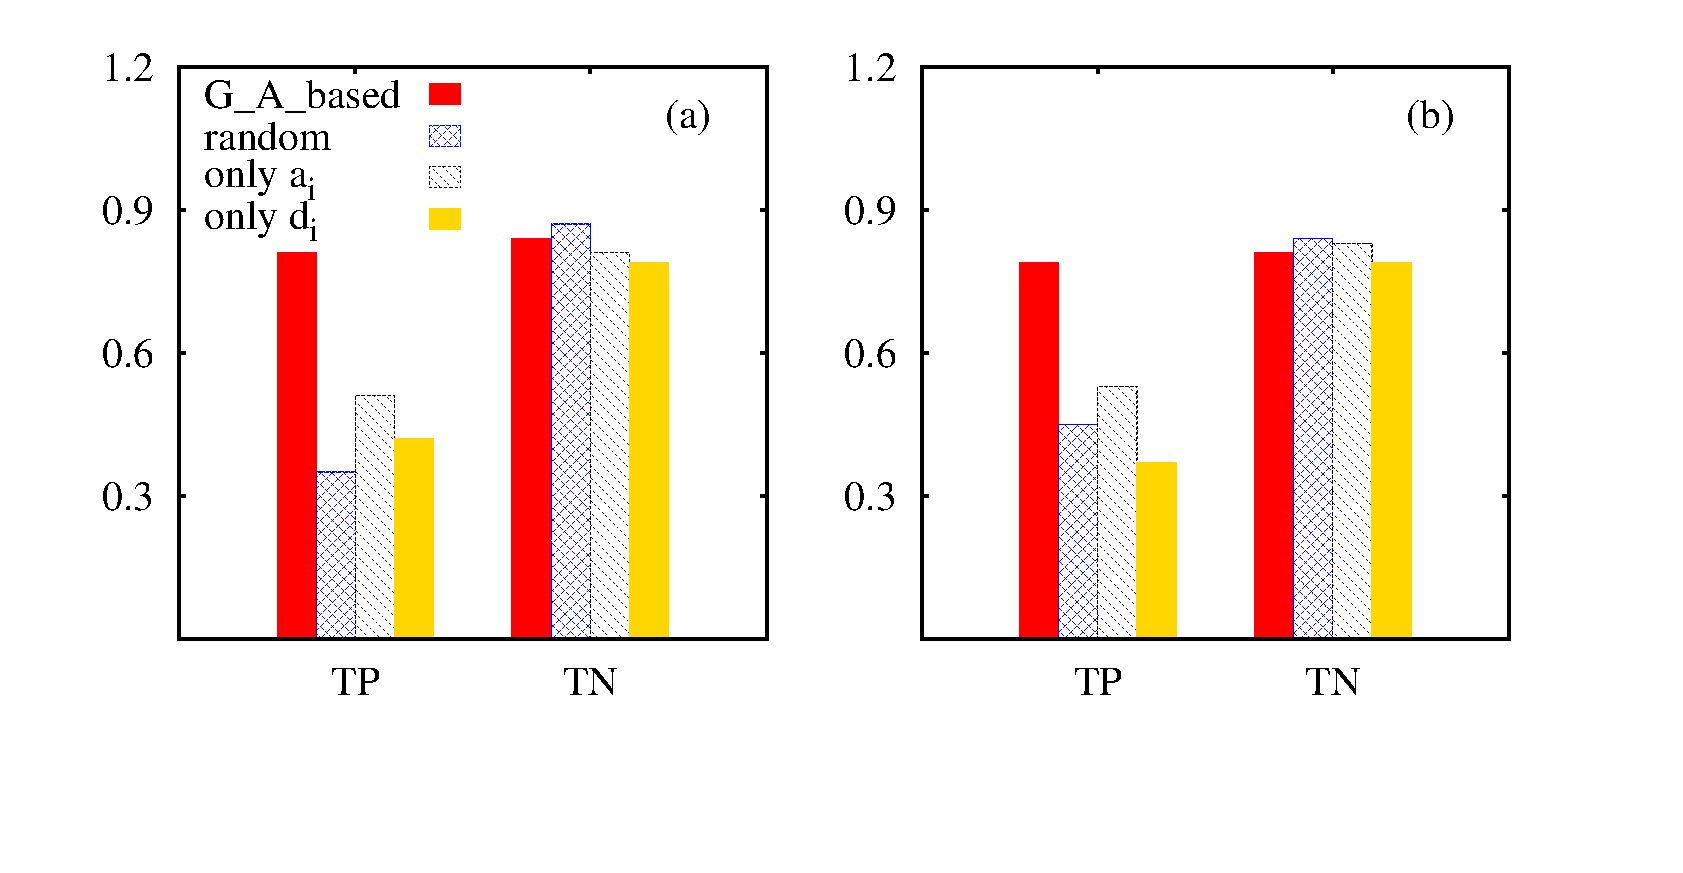
\includegraphics[scale = 0.35]{./texfiles/Chapter_4/cikm_17/figures/G_A_baseline.eps}
\caption{\label{fig:GA_base} Mean true positive (averaged over accepted and rejected papers) value with recommendation by our method (G\_A\_based) and the baseline. Results are 
noted for (a) JHEP and (b) JSTAT. $k = 15$.}
\end{figure}

\if{0}
\mycheck{Discard this part?}
\noindent{\bf{Further refinements:}} We observed in the previous section that under-performing reviewers when clubbed together often send in contradicting review reports. More specifically, 
reviewer class combinations of HH and LL contributes to a major proportion of discordant cases. We leverage this result and remove all the groups of class 
combinations HH and LL from the recommended set of reviewer groups. We observe that the size of the recommended set reduces on an average by 22.75\% for 
JHEP and around 22\% for JSTAT dataset (refer to figure \ref{fig:G_A_mod}). For JHEP dataset TP cases reduces to $76\%$ from $81\%$ for accepted and to $71.3\%$ 
from $75\%$ for rejected papers while the TN case improves to $86\%$ and $81\%$ for accepted and rejected papers respectively. The corresponding values for 
JSTAT dataset are $76\%$ ($79\%$), $71\%$ ($75\%$), $83\%$ ($81\%$) and $74\%$ ($71\%$). Hence with only very marginal change in accuracy we are able to recommend 
an even smaller set of reviewer groups. 

\begin{figure}
\includegraphics[scale = 0.26]{figures/G_A_all_mod.eps}
\caption{\label{fig:G_A_mod} True positive (TP) and true negative (TN) cases while recommending a set of reviewer groups for both accepted and rejected papers 
for (a) JHEP and (b) JSTAT after removing HH and LL reviewer class combinations. $k = 15$}
\end{figure}
\fi

\medskip
